% Note with new geometry paper has to be defined in preamble
% I do not feel very confident of this
% Don't understand it fully how is working
 %\@twosidefalse \@mparswitchfalse % one side option
\cxset{geometry oxford/.code={
\newgeometry{left=74.8mm,top=27.4mm,headsep=2\baselineskip,%
marginparsep=8.2mm,marginparwidth=49.4mm,textheight=49\baselineskip,headheight=\baselineskip}
\@twosidefalse \@mparswitchfalse % one side option
\reversemarginpar
}}

\cxset{geometry textwidth/.store in=\textwidth@cx,
          geometry textheight/.store in=\textheight@cx,
          geometry tufte/.code={
             \newgeometry{a4paper,left=24.8mm,top=27.4mm,headsep=2\baselineskip,%
             textwidth=107mm,marginparsep=8.2mm,marginparwidth=49.4mm,%
             textheight=\textheight@cx\baselineskip,headheight=\baselineskip}
            \@twosidefalse \@mparswitchfalse % one side option
           %\reversemarginpar
    }
}


\cxset{marginpar push/.store in=\marginparpush@cx,
          marginpar font/.store in=\marginparfont@cx,
          marginpar justification/.is choice,
          marginpar justification/justifying/.code=\gdef\marginparjustification@cx{\justifying},
          marginpar justification/raggedright/.code=\gdef\marginparjustification@cx{\raggedright},
          marginpar justification/RaggedRight/.code=\gdef\marginparjustification@cx{\RaggedRight},
          marginpar justification/RaggedLeft/.code=\gdef\marginparjustification@cx{\RaggedLeft},
 }
\cxset{marginpar push=10pt,
          marginpar font=\normalfont\footnotesize\sffamily,
          marginpar justification=RaggedLeft}

\cxset{style13, geometry textheight=47,
          geometry tufte,
          watermark text=SAMPLE TUFTE VARIANT,
          watermark text color=thered,
          header style=samplepage}

\@ifundefined{stockheight}{\newlength\stockheight}{}
\@ifundefined{stockwidth}{\newlength\stockwidth}{}

% This is a sidenote without the footnote mark
\newcommand\marginnote[2][0pt]{%
 % \let\cite\@tufte@infootnote@cite%   use the in-sidenote \cite command
  %\gdef\@tufte@citations{}%           clear out any old citations
  \@tufte@margin@par%                 use parindent and parskip settings for marginal text
  \marginpar{\hbox{}\vspace*{#1}\marginparfont@cx\marginparjustification@cx\vspace*{-1\baselineskip}\noindent #2}%
  \@tufte@reset@par%                  use parindent and parskip settings for body text
  %\@tufte@print@citations%            print any citations
  %\let\cite\@tufte@normal@cite%       go back to using normal in-text \cite command
}

% This macro has been adapted from the layouts package, it sets the units to be printed
% in the diagrams.
\newcommand{\printinunitsof@cx}[1]{%
  \def\l@yunitperpt{1.0}\def\l@yunits{pt}%
  \def\l@yta{#1}\def\l@ytb{pt}%
  \ifx \l@yta\l@ytb
    \def\l@yunitperpt{1.0}\def\l@yunits{pt}%
  \else
    \def\l@ytb{pc}%
    \ifx \l@yta\l@ytb
      \def\l@yunitperpt{0.083333}\def\l@yunits{pc}%
    \else
      \def\l@ytb{in}%
      \ifx \l@yta\l@ytb
        \def\l@yunitperpt{0.013837}\def\l@yunits{in}%
      \else
        \def\l@ytb{mm}%
        \ifx \l@yta\l@ytb
          \def\l@yunitperpt{0.351459}\def\l@yunits{mm}%
        \else
          \def\l@ytb{cm}%
          \ifx \l@yta\l@ytb
            \def\l@yunitperpt{0.0351459}\def\l@yunits{cm}%
          \else
            \def\l@ytb{bp}%
            \ifx \l@yta\l@ytb
              \def\l@yunitperpt{0.996264}\def\l@yunits{bp}%
            \else
              \def\l@ytb{dd}%
              \ifx \l@yta\l@ytb
                \def\l@yunitperpt{0.9345718}\def\l@yunits{dd}%
              \else
                \def\l@ytb{cc}%
                \ifx \l@yta\l@ytb
                  \def\l@yunitperpt{0.0778809}\def\l@yunits{cc}%
%                \else
%                  \def\l@ytb{PT}%
%                  \ifx \l@yta\l@ytb
%                    \def\l@yunitperpt{1.0}\def\l@yunits{PT}% gives problems with pgfmathparse
%                  \fi
                \fi
              \fi
            \fi
          \fi
        \fi
      \fi
    \fi
  \fi
}

% Define keys to set it
\cxset{geometry units/.code=\printinunitsof@cx{#1}}
\cxset{geometry units=pt}

% #1 value in pts
% default in mm sorry USA.
\def\convert@cx#1{%
   \pgfmathparse{#1*\l@yunitperpt}
   \pgfmathresult\thinspace\l@yunits
}

% Layout related macros to go to separate style file
\def\aspectratio{\pgfmathparse{\paperheight/\paperwidth} \pgfmathresult}
\newpage
\newlength\innermargin

\def\printgeometryvalues{%
   \noindent
   \cs{paperwidth} \convert@cx{\paperwidth}\\
   \cs{paperheight} \convert@cx{\paperheight}\\
   \cs{voffset} \convert@cx{\voffset}\\
   \cs{hoffset} \convert@cx{\hoffset}\\
   \cs{thetextheight}\convert@cx{\textheight}\\
   \cs{thetextwidth} \convert@cx\textwidth\\
   \cs{thetopmargin} \convert@cx{\topmargin}\\
   \cs{theheadheight} \convert@cx{\headheight}\\
   \cs{theheadsep} \convert@cx{\headsep}\\
   \cs{theoddsidemargin} \convert@cx{\oddsidemargin}\\
   \cs{theevensidemargin}\convert@cx{\evensidemargin}\\
   \cs{themarginparsep} \convert@cx{\marginparsep}\\
   \cs{themarginparwidth} \convert@cx{\marginparwidth}\\
   \cs{themarginpush} \convert@cx{\marginparpush}\\
   \cs{thevoffset} \convert@cx{\voffset}\\
   \cs{thefootskip} \convert@cx{\footskip}\\
   \cs{aspect ratio} \aspectratio\\
   twoside = \if@twoside true\else false\\
  reversemarginpar = \if@mparswitch true \else false\\
 }

\def\alignedge{%
  \checkoddpage%
  \parindent0pt%
%   \ifoddpage \global\setlength\innermargin{\oddsidemargin}
%          \else \global\setlength\innermargin{\evensidemargin}
%      \fi%
%   \if@twoside\setlength\innermargin{\dimexpr(\evensidemargin-\marginparsep)}%
%             \else\let\innermargin\oddsidemargin\fi
\ifoddpage \innermargin\oddsidemargin\else\innermargin\evensidemargin\fi
 }

% Set to true to draw an oddside page. Initially set to false.
\newcommand\layoutscale@cx{0.35}
\newif\ifoddpagelayout@cx
   \oddpagelayout@cxtrue
% Set true to draw marginpars on a page
\newif\ifdrawmarginpars
   \drawmarginparstrue

\checkoddpage
\alignedge

\def\printlayout{%
\pgfmathsetmacro\tol{5mm}


\def\innermarginname{%
   \ifoddpage oddsidemargin \else evensidemargin\fi
}
\begin{tikzpicture}[scale=\layoutscale@cx,font={\footnotesize\sffamily},line width=.8pt]
\checkoddpage
\alignedge
\coordinate (pageX1) at (0,\paperheight);
\coordinate (text1) at (1in+\innermargin,\paperheight-1in-\topmargin-\headsep-\headheight);
% origin
\draw [fill=black] (0,0) circle (3.5pt); 
% draw paper
\draw (pageX1) rectangle ++(\paperwidth, -\paperheight);
% draw one inch around
\draw [color=gray] (1in, 0) -- ++(0, \paperheight);
\draw [color=gray] (0, \paperheight-1in) -- ++ (\paperwidth,0);
% draw textarea
\draw [color=green] (text1) rectangle ++ (\textwidth ,-\textheight);
% oddside margin
\draw [color=NavyBlue] (1in+\innermargin, \paperheight-1in-\headsep-\headheight-\topmargin) -- ++ (0,-\textheight);
% marginpar
\ifdrawmarginpars
  \checkoddpage
    \ifoddpage
      \draw [color=black] (1in+\innermargin+\textwidth+\marginparsep,   \paperheight-1in-\topmargin-\headsep-\headheight ) rectangle ++(\marginparwidth,-\textheight);
    \else
      \draw [color=red] (1in+\innermargin-\marginparsep,\paperheight-1in-\topmargin-\headsep-\headheight ) rectangle ++(-\marginparwidth,-\textheight);
  \fi
\fi
% header
%   top margin
\draw [color=black] (1in + \innermargin+\tol, \paperheight-1in-\topmargin) 
               -- ++ (\textwidth,0);
\draw [color=black] (1in + \innermargin, \paperheight-1in-\topmargin ) 
               rectangle ++ (\textwidth,-\headheight);
% footer
\draw (1in+\innermargin,\paperheight-1in-\topmargin-\headheight-\headsep-\textheight-\footskip)
         -- ++ (\textwidth,0) rectangle ++ (-\textwidth,+\headheight);
\draw [color=gray] (0,1in)--(0+\paperwidth,1in);

%\iffalse
% legends and dimensions top x-axis
\draw (0,\paperheight+\tol)
        -- ++(0,.8) 
       ++ (1in, -0.8)
       -- ++(0,0.8) node[ above left]{1inch}; 
 \draw (-0.4,\paperheight+3mm+4mm) -- ++ (\paperwidth-\marginparwidth+2*\marginparsep,0);% horizontal line
 % back
\draw (0+1in,\paperheight+3mm)--++(0,8mm);
\draw (0+1in+\innermargin,\paperheight+3mm)--++(0,8mm)
         node[ right]{\innermarginname=\the\oddsidemargin};
% margin sep ticks
\draw (1in+\innermargin+\textwidth,\paperheight+\tol) -- ++ (0,20mm)++(0,-0.23) node [ left]{marginparsep=\the\marginparsep};
\draw (1in+\innermargin+\textwidth+\marginparsep,\paperheight+\tol) -- ++ (0,20mm);
% marginpar ticks
\draw (1in+\innermargin+\textwidth+\marginparsep+\marginparwidth,\paperheight+\tol) 
     -- ++ (0,20mm)
         ++ (-\marginparwidth-\marginparsep-\tol,-0.5cm)
     --  ++ (\marginparsep+\marginparwidth+4*\tol,0) ++(18mm,3mm) node {marginparwidth=\the\marginparwidth};
 % ticks on y-axis right
\draw (\paperwidth+\tol,\paperheight)
        -- ++ (0.8,0) 
        ++ (-0.8,-1in-\topmargin)
        --++(0.8,0)  node  [below right]{headheight = \the\headheight}
        ++ (-0.8,-\headheight) 
     -- ++(0.8,0)
        ++ (-0.8,-\headsep) -- ++ (0.8,0) node [above right]{headsep = \the\headsep}

        ++ (-0.8,-\textheight) -- ++ (0.8,0) node[right] at ++(0,0.5\textheight){textheight=\the\textheight}
        ++ (-0.8, -\footskip) -- ++ (0.8,0)node [above right]{footskip = \the\footskip}
        (\paperwidth+7mm,\footskip-3mm)-- ++ (0,\paperheight+0.4);  
% bottom dimensions
\draw (-3mm,- 10mm) -- ++(1in+1cm,0) node[above] at ++(-0.5in-0.5cm,0){1 inch}(1in,-8.3mm)--++(0,-0.8cm);  
\draw (0,-8mm)-- 
       ++(0, -2.5cm)++(\paperwidth,2.5cm)--++(0,-2.5cm); 
\draw (-3mm,-2.5cm)--++(\paperwidth+6mm,0);
\node[above] at (-3mm+0.5\paperwidth, -2.5cm) {paper width = \the\paperwidth};  
%% left tick marks
\draw (-3mm,0)-- (-1.3cm,0)++(0,\paperheight)--++(1cm,0);
\draw [color=blue] (-7.8mm, -0.4) -- (-7.8mm,\paperheight + 0.4cm);
% legend
\node[rotate=90] at (-12.8mm, 0.5\paperheight){paper height = \the\paperheight};
%\fi
\end{tikzpicture}
}




\chapter{Geometry and Page Dimensions}
\parindent1.5em
\section{Introduction}






\convert@cx{\paperwidth}{pc}



Setting up the page geometry, is normally done by the class or if adjustments need to be made, most authors will use the package geometry. If you need to view the geometry and the values of the document layour you can use the pkg{layouts}. This package offers a set of convenience key values for setting up geometry in order to enable authors to have a comprehensive style sheet.

\section{How to set geometry via this package}

\section{Viewing the page geometry}

The package offers a number of keys to set documents either document wide or locally to change page 
parameters or to view the frames. this is very similar to what the layouts and geometry packages offer. We do
however use TikZ for these diagrams.

To incorporate a layouts diagram we offer two macros \cs{printlayout} and \cs{printlayoutvalues}. Both have associated styling keys.
\medskip

\printgeometryvalues

\begin{figure}
  \printlayout
  \caption{Page layout of this page.}
\end{figure}

\subsection{Paper sizes}
Most people using LaTeX, will print on either a4paper or letterpaper sizes. If you going to bind the work it might be necessary to trip the paper a little bit during binding to make sure that the top and side of the book are not ragged. This is normally called the \textit{trim}. If the document is to be printed by a publishing house this might be done by the printer which will use a different size \textit{stock size}. They might also allow for two additional dimensions called the spinemargin or the foremargin\marginnote{The memoir class.}

\subsection{The page dimensions}

The page dimensions are shown in figure 1. We tried to cater for the common terminology of all the classes.

\subsection{Textheight}

When using \cs{flushbottom} LaTeX expects that the \cs{textheight} is such that a number of textlines in the body font will fit exactly into the height. If not, it issues an underfull vbox's message. LaTeX calculates these parameters when loading the class .clo files.
 
number of lines : \pgfmathparse{(\textheight-\topskip)/(\baselineskip)-1}\pgfmathresult

\expandafter\def\csname a4page\endcsname{1000pt}

\@nameuse{a4page}

%\setlength\textheight{530pt}

\pgfmathresult,  \the\textheight \the\baselineskip

\pgfmathparse{(49-1)*\baselineskip + \topskip} \pgfmathresult

\ifdim\stockheight=0pt\addtolength\stockheight{\paperheight}\fi
\addtolength\stockheight{3mm}


\ifdim\stockwidth=0pt\addtolength\stockwidth{\paperwidth}\fi
\addtolength\stockwidth{3mm}

stock height\the\stockheight\\
\the\stockwidth

\newlength\lefttrim
\newlength\bottomtrim
\setlength\lefttrim{0mm}
\setlength\bottomtrim{0mm}

\setlength\trimtop{5mm}
\setlength\trimedge{10mm}

\lipsum[1]

\printlayout
\newpage

\section{Allowing for trims}
\newpage

\tikzset{dim/.style = {>= latex,color=black}}
\begin{tikzpicture}[scale=0.5,font={\footnotesize\sffamily},line width=.8pt,every node={color=black}]
% draw stockwidth and stockheight
\draw [color=gray] (0,0) rectangle ++(\stockwidth,\stockheight);
% draw the paper 
\draw [color=NavyBlue,dashed]  (0+\lefttrim,\stockheight-\trimtop) rectangle ++ (\stockwidth-\lefttrim-\trimedge,-\stockheight+\trimtop+\bottomtrim);
% dimensions one more try
\cxset{geometry units=mm}
% paper width dimensions, better to change to a macro
% tol is the distance to dimension

% paper width
\edef\tol{-2.5\baselineskip}
\coordinate (A) at (0+\lefttrim,\tol);
\coordinate (B) at (\stockwidth-\trimedge,\tol);
\coordinate (C) at (0.5\stockwidth,\tol);
\draw[dim, |<->|] (A) -- (B); 
\node at (C) [yshift=0.5\baselineskip)]{paper width = \convert@cx{\paperwidth}};

% stockwidth
\edef\tol{-5\baselineskip}
\coordinate (BD) at (0,\tol);
\coordinate (BD2) at (\stockwidth,-5\baselineskip);
\draw[dim, |<->|] (BD) -- (BD2); 
\node at (BD)[yshift=0.5\baselineskip,xshift=0.25*\stockwidth]{stockwidth=\convert@cx{\stockwidth}} ;

% trimedge
\coordinate (D) at (\stockwidth-4\trimedge, 0.17\textheight);
\coordinate (E) at (\stockwidth,0.17\textheight);
\draw [dim,->|] (D) -- ++(3\trimedge,0);
\draw [dim,|<-|] (E) -- ++(3\trimedge,0) node at ++(0,0) [right,text width=2cm,color=black] {trim edge \convert@cx{\the\trimedge}};

% toptrim
\coordinate (F) at (0.9\stockwidth, \stockheight-\trimtop-8mm);
\coordinate (G) at (0.9\stockwidth, \stockheight-\trimtop);
\coordinate (H) at (0.9\stockwidth,\stockheight);
\draw (F)[dim,->|] -- (G);
\draw (H) -- ++ (0,8mm) -- ++ (5mm,0)[|<-|,>=latex] node [right] at ++ (0,0) {top trim = \convert@cx{\the\trimtop}};

% 1in offsets
\draw[dashed,color=gray] (1in,0) -- (1in,\stockheight);
\draw[dashed,color=gray] (0in,\stockheight-1in)-- ++ (\stockwidth,0);
% head
\coordinate (I) at (1in-\lefttrim+\evensidemargin,\stockheight-1in-\headheight-\topmargin);
\draw (I) rectangle ++ (\textwidth,\headheight);

\draw[dim,<->] (1.5in\tol,\stockheight) -- ++(0,-1in) node[above right] at ++ (0,0.5in) {1in + yoffset};


% textarea
\coordinate (J) at (1in-\lefttrim+\evensidemargin,\stockheight-1in-\headheight-\topmargin-\headsep-\textheight);
\draw (J) rectangle ++ (\textwidth,\textheight);

\draw[dim,|<->|] (1in-\lefttrim+\evensidemargin,0.75\textheight) -- ++(\textwidth, 0)  node at ++(-0.5\textwidth,0.5\baselineskip) {textwidth} node at ++ (-0.5\textwidth,-\baselineskip) {\convert@cx{\the\textwidth}};

% footer
\coordinate (I) at (1in-\lefttrim+\evensidemargin,\stockheight-1in-\headheight-\topmargin-\headsep-\textheight-\footskip);
\draw (I) rectangle ++ (\textwidth,\headheight);


% marginpar 
\ifdrawmarginpars
  \checkoddpage
    \ifoddpage
      \draw [color=black] (1in+\innermargin+\textwidth+\marginparsep,   \paperheight-1in-\topmargin-\headsep-\headheight ) rectangle ++(\marginparwidth,-\textheight);
    \else
      \draw [color=red] (1in+\evensidemargin-\marginparsep,\stockheight-1in-\topmargin-\headsep-\headheight ) rectangle ++(-\marginparwidth,-\textheight);
     \draw [dim,|<->|] (1in-\lefttrim+\evensidemargin-\marginparsep-\marginparwidth,0.75\textheight) -- ++ (\marginparwidth,0) node at ++(-0.5\marginparwidth,0.5\baselineskip) {marginpar} node at ++(-0.5\marginparwidth,-\baselineskip){\convert@cx{\the\marginparwidth}};
  \fi
\fi

\end{tikzpicture}





\end{document}
\subsection{Headers and footers}
A page may have two additional items, and usually has at least one of these. They are the
running header and running footer. If the page has a folio then it is located either in the
header or in the footer. The word ‘in’ is used rather lightly here as the folio may not be
actually in the header or footer but is always located at some constant relative position. A
common position for the folio is towards the fore-edge of the page, either in the header or
the footer. This makes it easy to spot when thumbing through the book. It may be placed
at the center of the footer, but unless you want to really annoy the reader do not place it
near the spine.

Often a page header contains the current chapter title, with perhaps a section title on
the opposite header, as aids to the reader in navigating around the book. Some books put
the book title into one of the headers, usually the verso one, but I see little point in that as
presumably the reader knows which particular book he is reading, and the space would
be better used providing more useful signposts.

\section{Floating parameters}



\end{document}
\lipsum[1-4]\marginnote[1pt]{\lorem
    \lorem}

\lipsum[1-2]

%% Stick the caption in the head might as well place the first picture also
\def\asidecaption{\parbox{4.2cm}{{\bfseries Image \thefigure}\par\lorem}%
  % \addtocontents{lof}{This is image 8}
}
\def\ps@caption{%
     \let\@oddfoot\@empty\let\@evenfoot\@empty%
    \def\@evenhead{%
        \begin{picture}(0,0)%
           \put(-150,-80){\asidecaption\par}%
            \stepcounter{figure}
           \put(-150,-370){\asidecaption}%
        \end{picture}%
      }%
    \let\@oddhead\@evenhead%
    \let\@mkboth\@gobbletwo%
    \let\chaptermark\@gobble%
    \let\sectionmark\@gobble%
 }

\def\ps@bigpicture{%
    \setlength\headheight{19cm}%
    \let\@oddfoot\@empty\let\@evenfoot\@empty%
    \def\@evenhead{%
         \begin{picture}(0,0)%
          \put(-149,0){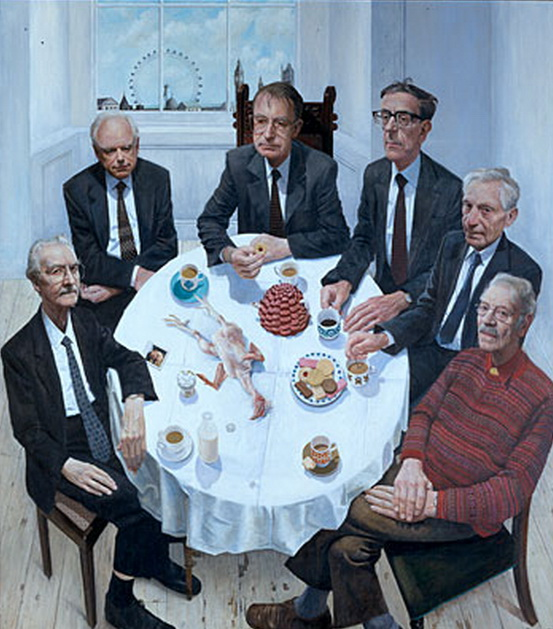
\includegraphics[width=\dimexpr(\textwidth+150pt)]{stuartpearson}}%
         \end{picture}%
      }%
    \let\@oddhead\@evenhead%
    \let\@mkboth\@gobbletwo%
    \let\chaptermark\@gobble%
    \let\sectionmark\@gobble%
 }


\def\doubletakeimage{%
  \renewcommand{\topfraction}{.95}  % ensure seecond image will not float away
  \begin{figure}[t]
    \thispagestyle{caption}
    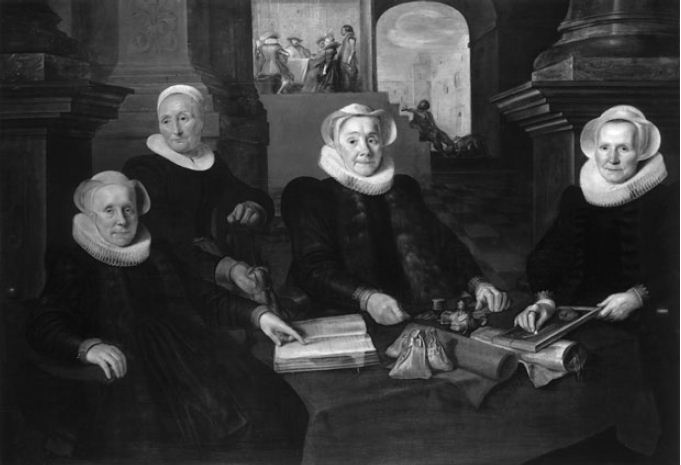
\includegraphics[width=\textwidth]{matron}%
  \end{figure}

  \begin{figure}[tp]
   \hspace*{-\marginparwidth}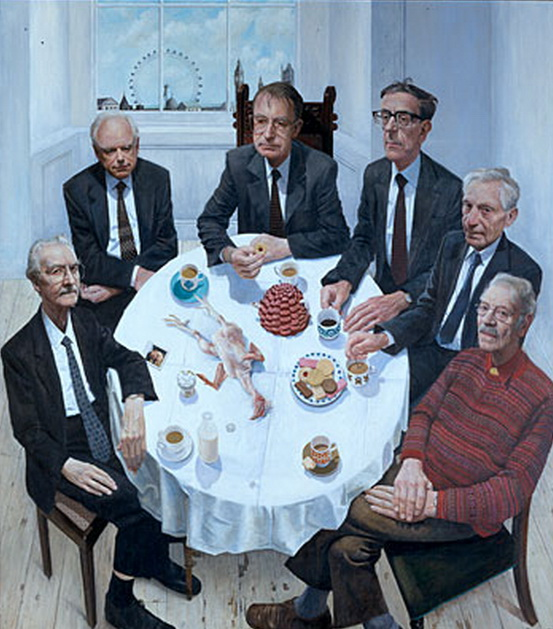
\includegraphics[height=0.9\textheight]{stuartpearson}
 \end{figure}
}


\doubletakeimage
\lipsum[1-4]
\begin{figure}[htp]
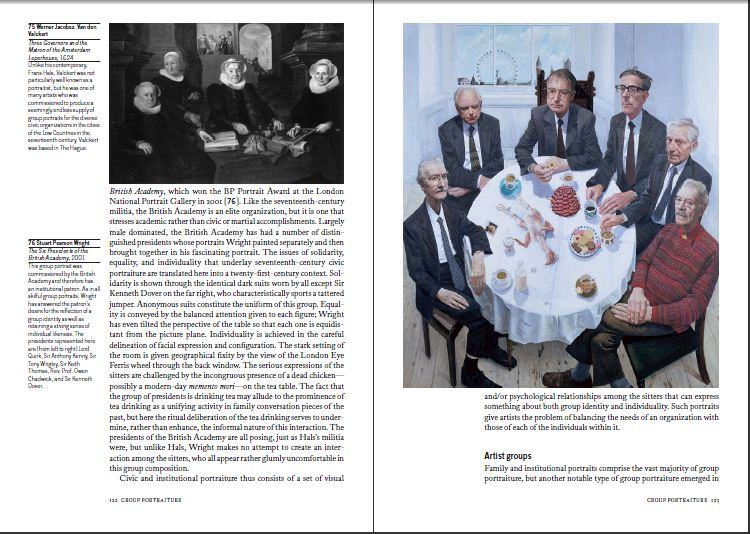
\includegraphics[width=0.98\textwidth]{captionspecial}
\centering
\caption{Figure from \textit{Oxford History of Art, Portraiture}, Shearer West, Oxford University Press, 2004. The figures are numbered consecutively and the text in the List of Illustrations have different formatting.}
\end{figure}
\restoregeometry
%% RESET EVERYTHING AT END OF CHAPTER
\addtocounter{chapter}{-2}
\@toctrue\@specialtrue
